\documentclass[12pt]{report}
\usepackage[utf8]{inputenc}
\usepackage[russian]{babel}
%\usepackage[14pt]{extsizes}
\usepackage{listings}

% Для листинга кода:
\lstset{ %
language=java,                 % выбор языка для подсветки 
basicstyle=\small\sffamily, % размер и начертание шрифта для подсветки кода
numbers=left,               % где поставить нумерацию строк (слева\справа)
numberstyle=\tiny,           % размер шрифта для номеров строк
stepnumber=1,                   % размер шага между двумя номерами строк
numbersep=5pt,                % как далеко отстоят номера строк от подсвечиваемого кода
showspaces=false,            % показывать или нет пробелы специальными отступами
showstringspaces=false,      % показывать или нет пробелы в строках
showtabs=false,             % показывать или нет табуляцию в строках            
tabsize=2,                 % размер табуляции по умолчанию равен 2 пробелам
captionpos=t,              % позиция заголовка вверху [t] или внизу [b] 
breaklines=true,           % автоматически переносить строки (да\нет)
breakatwhitespace=false, % переносить строки только если есть пробел
escapeinside={\#*}{*)}   % если нужно добавить комментарии в коде
}

% Для измененных титулов глав:
\usepackage{titlesec, blindtext, color} % подключаем нужные пакеты
\definecolor{gray75}{gray}{0.75} % определяем цвет
\newcommand{\hsp}{\hspace{20pt}} % длина линии в 20pt
% titleformat определяет стиль
\titleformat{\chapter}[hang]{\Huge\bfseries}{\thechapter\hsp\textcolor{gray75}{|}\hsp}{0pt}{\Huge\bfseries}

\usepackage{amsmath}
\usepackage{mathptmx}
% plot
\usepackage{pgfplots}
\usepackage{filecontents}
\usepackage{amsmath}
\usepackage{tikz,pgfplots}
\usetikzlibrary{datavisualization}
\usetikzlibrary{datavisualization.formats.functions}

\usepackage{geometry}
\geometry{verbose, a4paper,tmargin=2cm, bmargin=2cm, rmargin=1.5cm, lmargin = 3cm}

\usepackage{graphicx}
\graphicspath{{src/}}
\DeclareGraphicsExtensions{.pdf,.png,.jpg}

\begin{document}
%\def\chaptername{} % убирает "Глава"
\begin{titlepage}
	\centering
	{\scshape\LARGE МГТУ им. Баумана \par}
	\vspace{3cm}
	{\scshape\Large Рубежный контроль №2\par}
	\vspace{0.5cm}	
	{\scshape\Large По курсу: "Анализ алгоритмов"\par}
	\vspace{1.5cm}
	{\huge\bfseries Регулярные выражения \par}
	\vspace{2cm}
	\Large Работу выполнил: Лумбунов Дмитрий, ИУ7-54\par
	\vspace{0.5cm}
	\Large Преподаватели:  Волкова Л.Л., Строганов Ю.В.\par

	\vfill
	\large \textit {Москва, 2019} \par
\end{titlepage}

\tableofcontents

\newpage
\chapter*{Введение}
\addcontentsline{toc}{chapter}{Введение}

Цель работы: изучение возможностей регулярных выражений. Реализация валидации строк при использовании регулярных выражений и конечного автомата.
В ходе рубежного контроля предстоит:
\begin{itemize}
	\item Изучить регулярные выражения; 
	\item реализовать алгоритм валидации строк формата даты с помощью регулярных выражений и конечного автомата.
\end{itemize}

\chapter{Аналитическая часть}
Регулярные выражения (англ. regular expressions) — формальный язык поиска и осуществления манипуляций с подстроками в тексте, основанный на использовании метасимволов (символов-джокеров, англ. wildcard characters). Для поиска используется строка-образец (англ. pattern, по-русски её часто называют «шаблоном», «маской»), состоящая из символов и метасимволов и задающая правило поиска. Для манипуляций с текстом дополнительно задаётся строка замены, которая также может содержать в себе специальные символы.


\section{Использование регулярных выражений}
Регулярные выражения используются некоторыми текстовыми редакторами и утилитами для поиска и подстановки текста. Например, при помощи регулярных выражений можно задать шаблоны, позволяющие:
\begin{itemize}
	\item найти все последовательности символов «кот» в любом контексте, как то: «кот», «котлета», «терракотовый»;
	\item найти отдельно стоящее слово «кот» и заменить его на «кошка»;
	\item найти слово «кот», которому предшествует слово «персидский» или «чеширский»;
	\item убрать из текста все предложения, в которых упоминается слово кот или кошка.
\end{itemize}
Регулярные выражения позволяют задавать и гораздо более сложные шаблоны поиска или замены.

Результатом работы с регулярным выражением может быть:
\begin{itemize}
	\item проверка наличия искомого образца в заданном тексте;
	\item определение подстроки текста, которая сопоставляется образцу;
	\item определение групп символов, соответствующих отдельным частям образца.
\end{itemize}
Если регулярное выражение используется для замены текста, то результатом работы будет новая текстовая строка, представляющая из себя исходный текст, из которого удалены найденные подстроки (сопоставленные образцу), а вместо них подставлены строки замены (возможно, модифицированные запомненными при разборе группами символов из исходного текста). Частным случаем модификации текста является удаление всех вхождений найденного образца — для чего строка замены указывается пустой.
\section{Регулярные выражения в теории формальных языков}
Регулярные выражения состоят из констант и операторов, которые определяют множества строк и множества операций на них соответственно. Определены следующие константы:
\begin{itemize}
\item (пустое множество) $\emptyset$.
\item (пустая строка) $\epsilon$ обозначает строку, не содержащую ни одного символа; эквивалентно \"".
\item (символьный литерал) "a", где a — символ используемого алфавита.
\item (множество) из символов, либо из других множеств.
и следующие операции:
\end{itemize}
\begin{itemize}
	\item (сцепление, конкатенация) RS обозначает множество ${\alpha\beta | \alpha \in R  \& \beta \in S}$. Например, \{"boy", "girl"\}\{"friend", "cott"\} = \{"boyfriend", "girlfriend", "boycott", "girlcott"\}.
	\item(дизъюнкция, чередование) $R|S$ обозначает объединение R и S.
	
	 Например, \{"ab", "c"\}|\{"ab", "d", "ef"\} = \{"ab", "c", "d", "ef"\}.
	\item(замыкание Клини, звезда Клини) R* обозначает минимальное надмножество множества R, которое содержит $\epsilon$ и замкнуто относительно конкатенации. Это есть множество всех строк, полученных конкатенацией нуля или более строк из R.
	
	 Например, \{"Run", "Forrest"\}* = \{$\epsilon$, "Run", "Forrest", "RunRun", "RunForrest", "ForrestRun",
	 
	  "ForrestForrest", "RunRunRun",
	
	 "RunRunForrest", "RunForrestRun", \}.
	\item Регулярные выражения, входящие в современные языки программирования (в частности, PCRE), имеют больше возможностей, чем то, что называется регулярными выражениями в теории формальных языков; в частности, в них есть нумерованные обратные ссылки. Это позволяет им разбирать строки, описываемые не только регулярными грамматиками, но и более сложными, в частности, контекстно-свободными грамматиками.
\end{itemize}
\section{Вывод}
Были рассмотренны регулярные выражения и их обоснование в теории формальных языков.

\chapter{Конструкторская часть}
\section{Требования к программе}
\textbf{Требования к вводу:}
\begin{itemize}
	\item на вход подается строка;
	\item длина входной строки не превышает максимально допустимую длину для типа String ЯП Java.
\end{itemize}
\textbf{Требования к программе:}
\begin{itemize}
	\item Программа выводит входные строки и результат валидации по конечному автомату (valid/invalid);
	\item программа выводит результат валидации по регулярным выражениям (true/false).
\end{itemize}

\section{Конечный автомат}
В этом разделе будет рассмотрен конечный автомат, на котором основан алгоритм (Рис. \ref{fig:avt})

\begin{figure}[h]
	\center{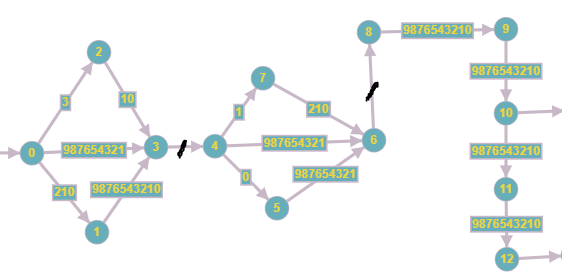
\includegraphics[scale=0.9]{graph.png}} 
	\caption{Конечный автомат для формата даты}
	\label{ris:example}
\end{figure}

\section{Вывод}
В данном разделе был рассмотрен конечный автомат, на котором основан алгоритм и требования к работе программы.

\chapter{Технологическая часть}
\section{Выбор ЯП}
Я выбрал в качестве языка программирования Java, потому как он данный язык имеет поддержку регулярных выражений и удобен при объектно-ориентированном подходе.

\section{Листинг кода алгоритмов}
В данном разделе будет представлен листинги кода валидации с помощью регулярных выражений (\ref{RegExp}), с помощью конечного автомата(\ref{Avt})
\begin{lstlisting}[label=RegExp,caption = Использование регулярных выражений]

import java.util.regex.Pattern;

String[] Str = new String[5];
Str[0] = "31/12/01"; Str[1] = "1/3/1925"; Str[2] = "5/5,12"; Str[3] = "32/1/09"; Str[4] = "30.13.2012";

for (int i = 0; i < Str.length; i++){
    System.out.println(Pattern.matches("(0?[1-9]|[12][0-9]|3[01])/(0?[1-9]|1[012])/((\\d{2})|(\\d{4}))",Str[i]));
}

\end{lstlisting}

\begin{lstlisting}[label=Avt,caption=Использование конечного автомата]


class Date {
    
    byte day;
    byte month;
    short year;
    char delimiter;
    
    static Date stringToDate (String str) {
        String temp = "";
        int i = 0;
        
        Date Ret = new Date();
        
        //day
        for ( ; Character.isDigit(str.charAt(i)) && i < str.length(); i++){
            temp += str.charAt(i);
        }
        
        
        //no delimiter
        if (i == str.length()) return null;
        
        //not value
        for (int j = 0; j < temp.length(); j++){
            if (!Character.isDigit(temp.charAt(j))) return null;
        }
        
        
        //length
        if (1 > temp.length() || temp.length() > 2) return null;
        
        //saving
        Ret.day = Byte.parseByte(temp);
        Ret.delimiter = str.charAt(i);
        if (Ret.day > 31 || Ret.day < 1) return null;
        temp = "";
        
        i++;
        
        //month
        for ( ; Character.isDigit(str.charAt(i)) && i < str.length(); i++){
            temp += str.charAt(i);
        }
        
        
        //no second delimiter
        if (i == str.length() || str.charAt(i) != Ret.delimiter) return null;
        
        //not value
        for (int j = 0; j < temp.length(); j++){
            if (!Character.isDigit(temp.charAt(j))) return null;
        }
        
        //length
        if (1 > temp.length() || temp.length() > 2) return null;
        
        //saving
        Ret.month = Byte.parseByte(temp);
        if (Ret.month > 12 || Ret.month < 1) return null;
        temp = "";
        
        i++;
        //year
        for ( ; i < str.length(); i++){
            temp += str.charAt(i);
        }
        
        //not value
        for (int j = 0; j < temp.length(); j++){
            if (!Character.isDigit(temp.charAt(j))) return null;
        }
        
        //length
        if (2 != temp.length() && temp.length() != 4) return null;
        
        //saving
        Ret.year = Short.parseShort(temp);
        
        
        return Ret;
         
    }
}


\end{lstlisting}


\section{Вывод}
В данном разделе была рассмотрена структура ПО и листинги кода программы.


\chapter*{Заключение}
\addcontentsline{toc}{chapter}{Заключение}
В ходе лабораторной работы были изучены возможности регулярных выражений. Были реализованы алгоритмы валидации строки при помощи регулярных выражений и конечного автомата.


\addcontentsline{toc}{chapter}{Список литературы}
\begin{thebibliography}{3}
	\bibitem{Fridl}
	Фридл, Дж. Регулярные выражения = Mastering Regular Expressions. — СПб.: «Питер», 2001. — 352 с. — (Библиотека программиста). 	\bibitem{Smith}
	Смит, Билл. Методы и алгоритмы вычислений на строках (regexp) = Computing Patterns in Strings. — М.: «Вильямс», 2006. — 496 с.
	\bibitem{Fort}
	Форта, Бен. Освой самостоятельно регулярные выражения. 10 минут на урок = Sams Teach Yourself Regular Expressions in 10 Minutes. — М.: «Вильямс», 2005. — 184 с.
\end{thebibliography}

\end{document}